\chapter{Evaluation}
\label{ch:evaluation}

This chapter details the evaluation process of the PIO device and SoC. Simulation was utilised as the primary verification technique, both through unit tests and testbenches, and through inspecting the output of example programs. Test software running on the SoC is also utilised.

FPGA Synthesis results are also presented, including utilisation and timing, and compared with current state of the art I/O hardware.

\section{Testbenches}

The primary tool used for verification is ChiselTest\footnote{\url{https://github.com/ucb-bar/chiseltest}}, introduced in Chapter \ref{ch:background}. For each module, unit test-style testbenches are written to verify that the hardware functioned as expected. ChiselTest uses Treadle\footnote{\url{https://github.com/chipsalliance/treadle}}, a high performance FIRRTL execution engine, as it's simulator backend by default. Treadle is used for simulation of the Chisel modules within the design, but does not include support for Verilog.

For modules written in Verilog, ChiselTest can still be used as the modules were wrapped as Chisel \txt{BlackBox} classes. ChiselTest can also target Verilator, a simulation tool that compiles Verilog to a high-performance cycle-accurate C++ model \cite{verilator}. Verilator has a longer startup time than Treadle due to the extra compilation steps involved, but is much faster, especially for larger designs. Verilator is used for the simulation of the full PIO device, as well as for unit testing of Verilog modules.


\begin{listing}[h!]
    \vspace{0.5cm}
    \begin{minted}{scala}
class ScratchRegTest extends AnyFlatSpec with 
  ChiselScalatestTester {
    "scratch register" should "read and write" in {
    test(new ScratchReg) { uut =>
    uut.io.write.data.poke(42)
    uut.io.write.enable.poke(true)
    uut.io.read.expect(0, "Clock not yet stepped, output should be 0")
    uut.clock.step()
    uut.io.read.expect(42, "Clock stepped, value 42 should be written")
    uut.io.write.data.poke(67)
    uut.clock.step()
    uut.io.read.expect(67, "Clock stepped with write enable still high, value 67 should be written")
    uut.io.write.enable.poke(false)
    uut.io.write.data.poke(78)
    uut.clock.step()
    uut.io.read.expect(67, "Clock stepped with write enable low, value 67 should remain")
    uut.clock.step(10)
    uut.io.read.expect(67, "Clock stepped with write enable low, value 67 should remain")
    }
    }
}
    \end{minted}
    \caption{An example test bench, used for testing the scratch register module.}
    \label{lst:test}
\end{listing}

An example unit test using ChiselTest is shown in Listing \ref{lst:test}. The primary method for verifying designs is by `poking' (setting) and `peeking' (reading) ports on the unit under test (\txt{uut}) while stepping the clock, and using \txt{expect} to make assertions about what the output should be. If the value in an \txt{expect} call does not match what the output, then the given error message, along with the failure of the location, is printed to assist with debugging. Waveform outputs of simulations can also be dumped to files for further inspection and debugging. An example test run for the scratch register test suite is show in Figure \ref{fig:testrun}, with both examples of passing and failing tests when invoked using sbt.

The codebase includes 52 unit unit tests, with at least one testbench for each module, which provides confidence in the correctness of the designs. Tests were mostly written before or alongside the modules themselves.

\begin{figure}[H]
    \centering
    \subfloat[\centering Passing]{{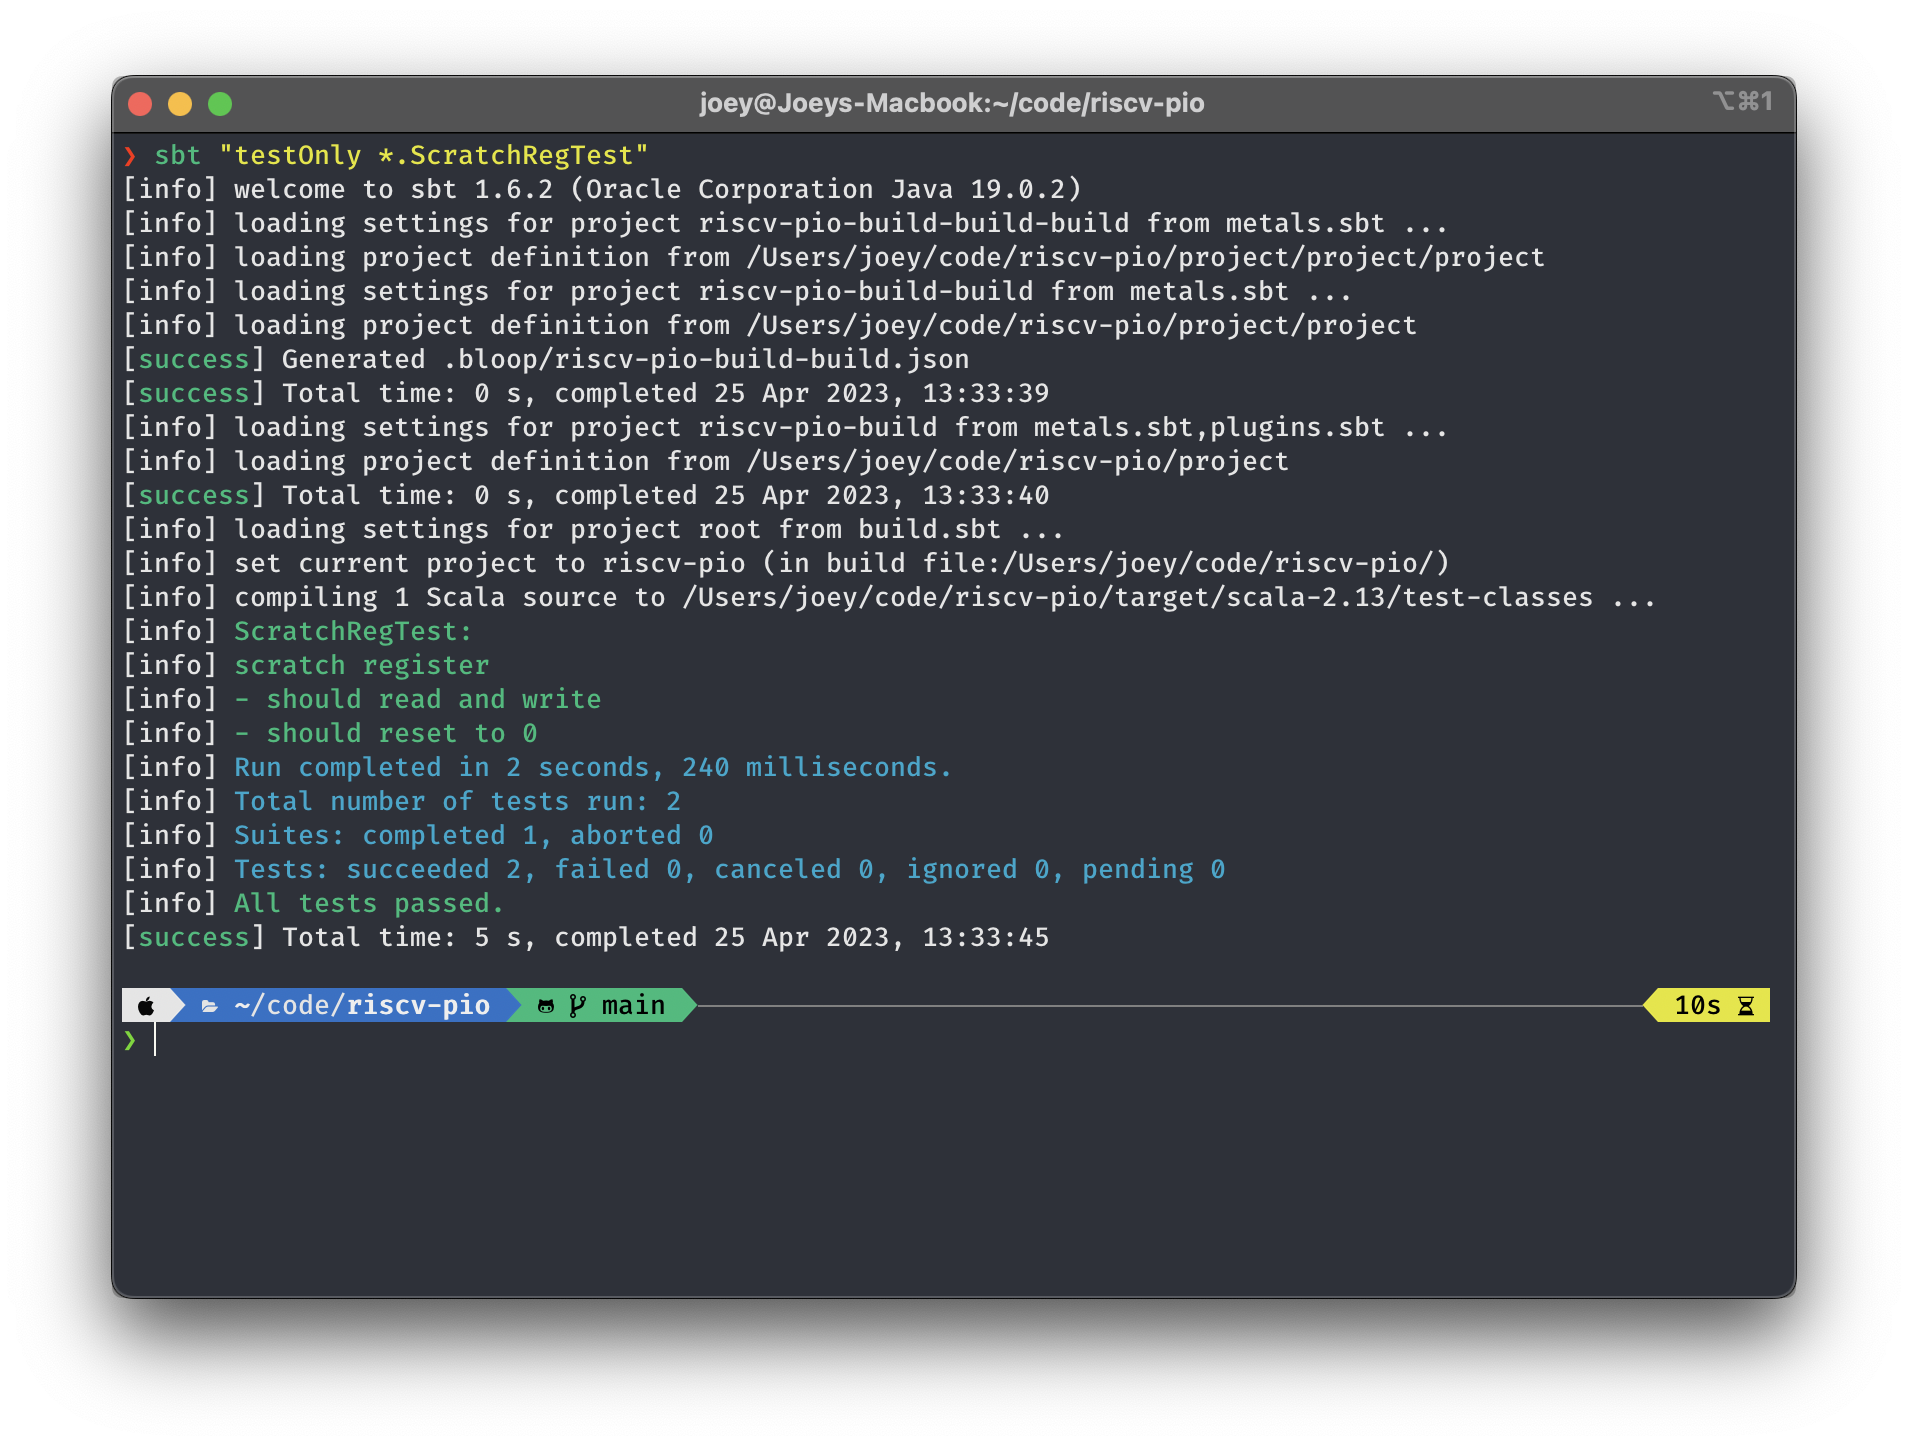
\includegraphics[width=0.45\textwidth]{../img/test-pass.png}} }
    \qquad
    \subfloat[\centering Failing]{{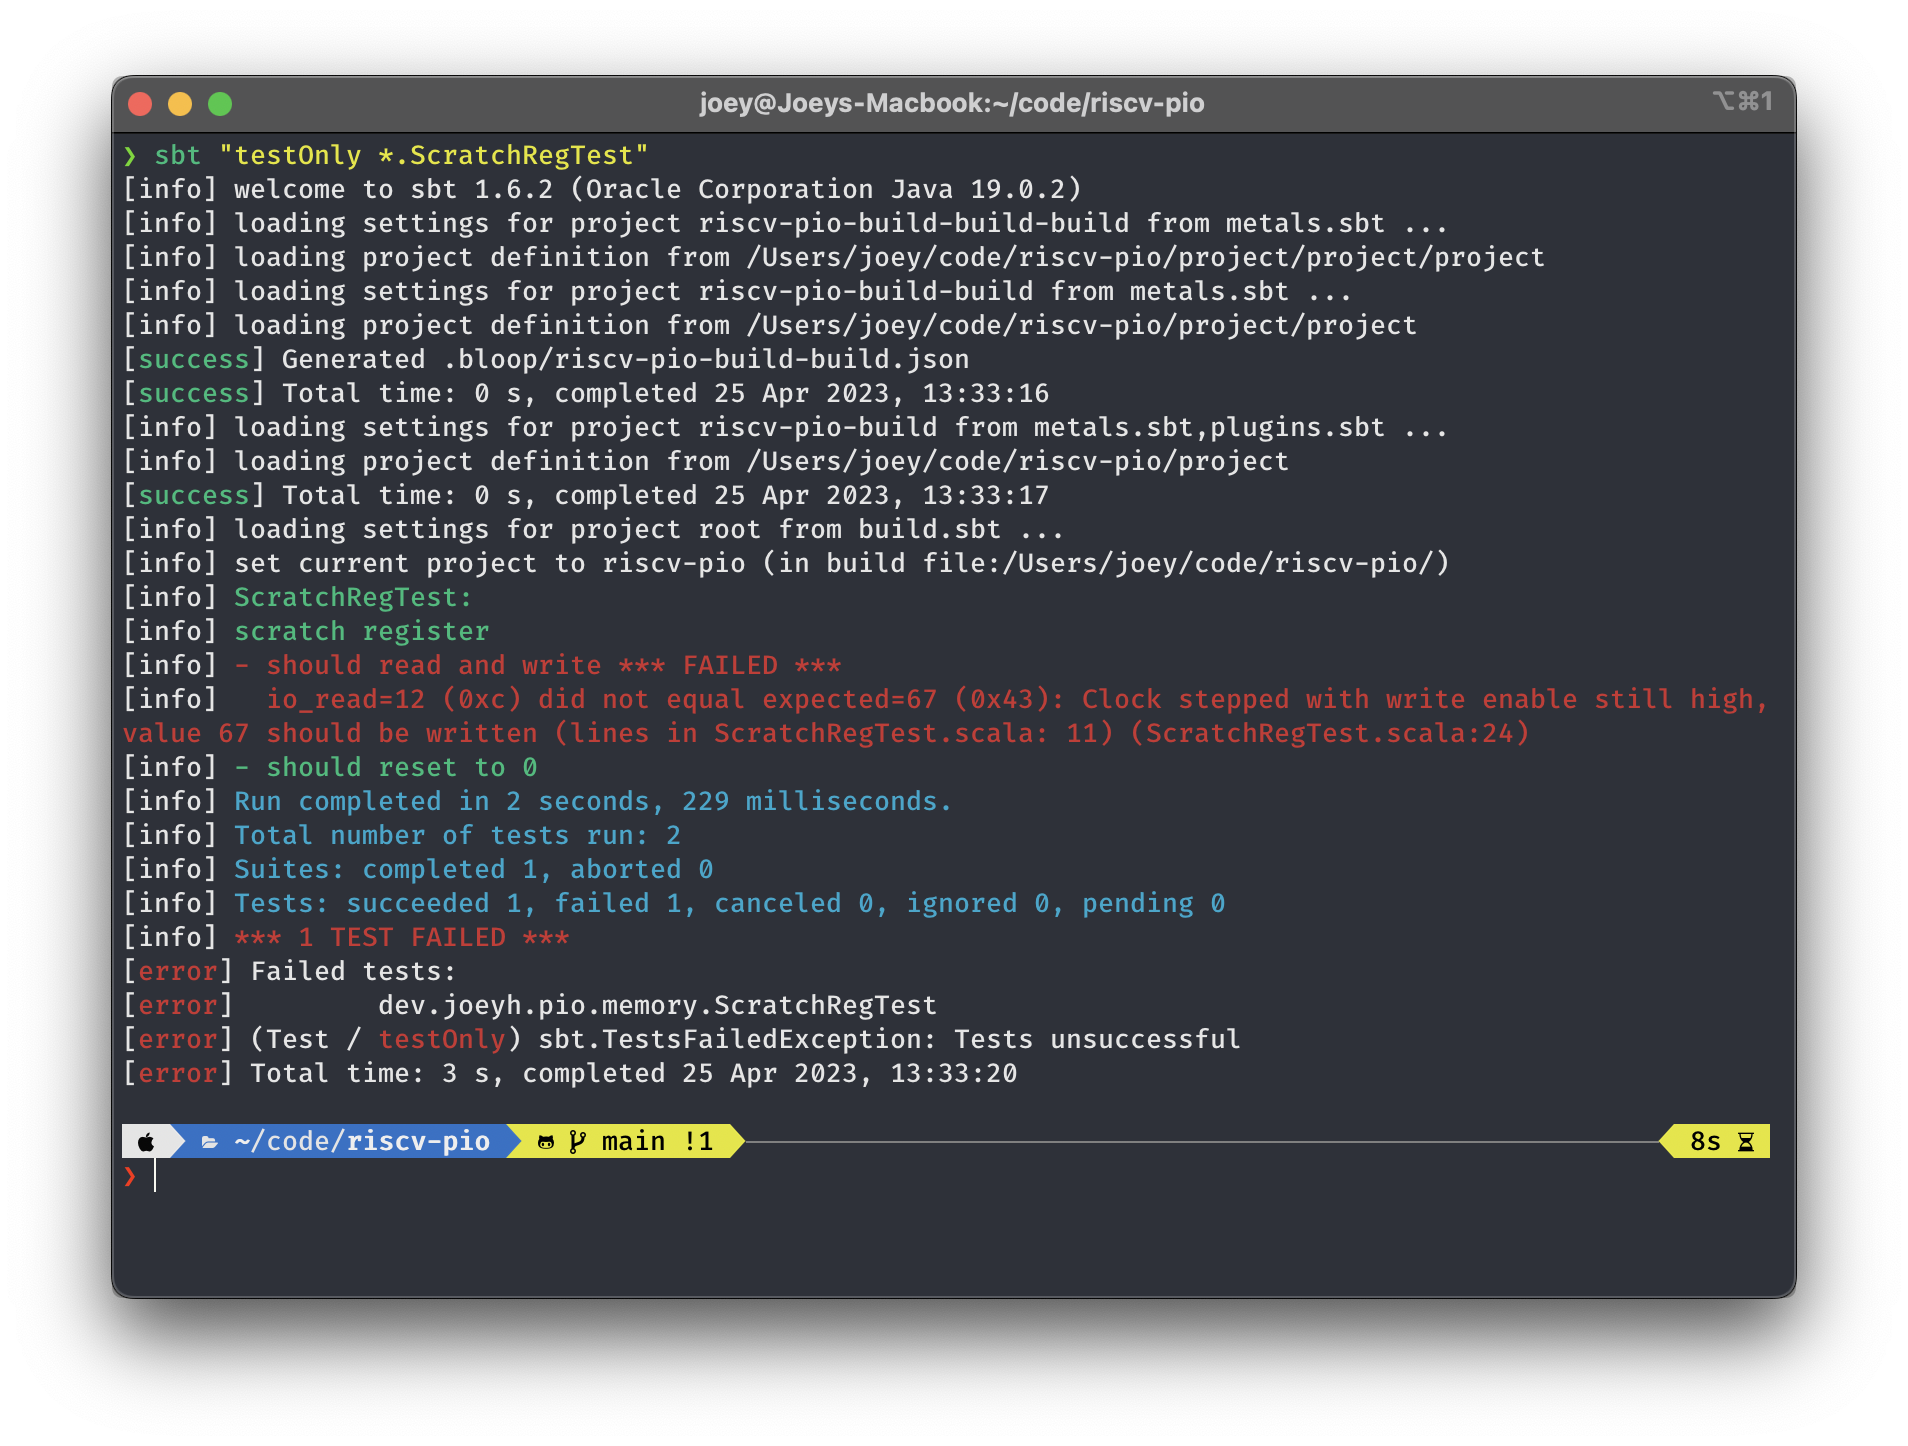
\includegraphics[width=0.45\textwidth]{../img/test-fail.png} }}
    \caption{Example outputs of test runs, invoked using sbt.}
    \label{fig:testrun}
\end{figure}


\section{Simulation \& Example Programs}
A full simulation of the PIO block can be ran using a ChiselTest testbench for the top level PIO module, which then allows to interact with the PIO block the same as the SoC would. The memory port is used to write a program and set control registers, and then the clock is ran for a number of cycles. Instead of making assertions about the expected behaviour on a cycle-accurate level, the test waveforms are dumped to a file for manual inspection to verify that the system as a whole is functioning as expected. All internal signals can be inspected, allowing to verify the interactions between internal components as well as the correctness of the outward-facing behaviour.

\begin{listing}[h!]
    \begin{minted}{scala}
//an example program
val program = Seq(
    "b111_0_0001_110_00001".U,
    "b111_0_0000_110_00000".U, 
    "b000_0_0000_000_00000".U  
)
uut.io.rw.write.enable.poke(true)
//write each instruction
program.zip(Seq(0.U, 1.U, 2.U)).foreach {
case (a, i) =>
    uut.io.address.poke(i)
    uut.io.rw.write.data.poke(a)
    uut.clock.step()
}
    \end{minted}
    \caption{Sample code to write a program to PIO memory in simulation}
    \label{lst:sim-write-prog}
\end{listing}

Three example PIO programs are presented: a square wave, an SPI interface, and WS2812B serial.

\subsection{Square Wave}

This is the most basic example, setting a pin high and then low in a loop to create a square wave that can be used to, for example, blink an LED.

\begin{listing}[h!]
    \begin{minted}{asm}
loop:
SET PINS, 1 [1]  //set output pin high, delay 1 cycle
SET PINS, 0      //set output pin low
JMP loop         //jump back to top
    \end{minted}
    \caption{RVPIO program to blink an LED}
    \label{lst:blinky}
\end{listing}


\subsection{WS2812B}

WS2812B intro

good use case because

show program

discuss config and timings

show waveform


\subsection{SPI}

SPI used for xyz
real interface
code
config


\section{Test Software}

Test software is used to verify that the SoC as implemented on the FPGA functions correctly, and to demonstrate that the test programs work outside simulation, The software is written in Rust, and includes support for both the UART device to provide a serial console, and the PIO device.

The PIO device is modelled in software as shown in Listing \ref{lst:pio-rs}. We make use of the \txt{volatile_register}\footnote{\url{https://github.com/japaric/volatile-register}} library for abstracting over write-only device registers. The library provides the \txt{WO<T>} type with a single method, \txt{write(&mut self, value: T)} for performing a volatile write to the register. Volatile writes are needed to prevent certain optimisations\footnote{Rust has no formal memory model so the exact semantics of a volatile operation are not strictly defined. At the time of writing, the compiler is guaranteed not to relatively re-order or elide any volatile writes, and the semantics are similar to as defined by the C11 standard \cite{rust_pointer, c11}} by the compiler which may cause issues when working directly with hardware registers.

All of the registers are represented within a single struct, which when accessed through the correct pointer, provides access to the hardware pointers. Writing to raw pointers is an unsafe operation in Rust, and is only permitted by the compiler within explicitly marked \txt{unsafe} code blocks or functions. We make use of an unsafe function to construct the \txt{Pio} object, by casting the address which the registers are located at to the struct type, and then converting that to a static reference which is stored in a wrapper struct.

\begin{listing}[h!]
    \begin{minted}{rust}
const PIO_ADDR: usize = 0x6004_0000;
pub struct Pio(&'static mut PioRegisters);
#[repr(C)]
struct PioRegisters {
    instructions: [WO<u32>; 32],
    clock_div: WO<u32>,
    branch_pin: WO<u32>,
    wrap_config: WO<u32>,
    input_pin_config: WO<u32>,
    output_pin_config: WO<u32>,
    isr_config: WO<u32>,
    osr_config: WO<u32>,
    enable: WO<u32>,
}
impl Pio {
    pub unsafe fn new() -> Self {
        Pio((PIO_ADDR as *mut PioRegisters)
            .as_mut()
            .unwrap())
    }
    pub fn enable(&mut self) {
        unsafe { self.0.enable.write(1); }
    }
}
    \end{minted}
    \caption{Software model of the PIO hardware}
    \label{lst:pio-rs}
\end{listing}

The example program that we run is the square wave one, to blink an LED on the FPGA board. The code to run the program is not dissimilar to the simulation: write the program and configuration to the registers and then enable the PIO. The function is shown in Listing \ref{lst:blink-sw}. The function uses \txt{unsafe} blocks to perform register writes, as the compiler cannot guarantee that the write to the hardware is always valid.

\begin{listing}[h!]
    \begin{minted}{rust}
pub fn blink(pio: &mut Pio) {
    let program: [u32; 3] = [
        0b111_0_0001_110_00001,
        0b111_0_0000_110_00000,
        0b000_0_0000_000_00000,
    ];
    unsafe {
        for (a, i) in program.iter().enumerate() {
            pio.0.instructions[a].write(*i);
        }
        pio.0.wrap_config.write(0b1_00000_00011_00000);
        pio.0.osr_config.write(0b_11000_1_1);
    }
    pio.enable();
}
    \end{minted}
    \caption{Rust function to initalise the PIO hardware with the square wave program in Listing \ref{lst:blinky}}
    \label{lst:blink-sw}
\end{listing}

The software is compiled to a static library using Cargo and Rustc, and then linked with some startup assembly code to call the main function using GCC. The linker also uses a linker script to lay out the binary in the correct way for the included bootloader to understand. The startup code, linker script and bootloader are provided by the same GitHub repository that provided the base SoC design.

The software and PIO both function as expected, blinking the configured LED on the FPGA board.

\section{Synthesis Results}
stuff from pres, maybe discuss timing a bit more??

\section{Comparison with existing I/O hardware}
the hard bit comparing state of the art
